\section{Summary of Paper \ref{pap:ikeda}}
\subsection*{"\nameref{pap:ikeda}"}
\subsection*{Scope and motivations}
An explicit semi-empirical formula was proposed in Paper \ref{pap:rolldamping}, based on a simplified version of Ikeda's method \cite{kawaharaSimplePredictionFormula2011}. This is a very low computational cost alternative. However, it was also found to have poor accuracy, especially for modern ship designs. 
Paper \ref{pap:ikeda} proposed a new hybrid method to address the shortcoming, where the viscous roll damping from Ikeda’s semi-empirical method was injected into an existing 3D unsteady fully nonlinear potential flow (FNPF) method \cite{kjellbergFullyNonlinearUnsteady2013}.

\subsection*{Results and main findings}
Viscous roll damping was calculated using Ikeda's method \cite{ikedaComponentsRollDamping1978} for the KVLCC2 test case. An error was encountered in the calculation of the $C_r$ coefficient used to obtain the eddy damping at zero speed. The source of this error was traced to a regression formula from experiments conducted by \textcite{ikedaEddyMakingComponent1978} on several two-dimensional cylinders with various sections. A new regression was instead proposed, using a decision tree model.
Fig.\ref{fig:ikeda_sections} shows $C_r$ from the experiments and corresponding predictions with Ikeda's method and the decision tree. The capital letters refer to cylinder sections from the experiments
\cite{ikedaEddyMakingComponent1978}.
\begin{figure}[h]
\center
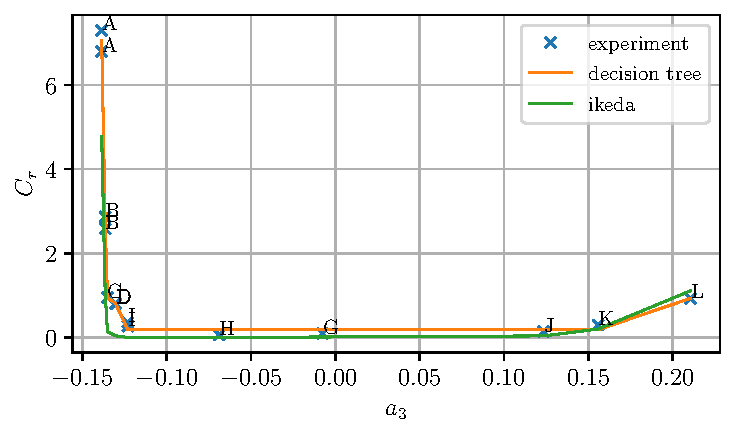
\includegraphics[width=\textwidth]{figures/ikeda_sections.pdf}
\vspace{-0.4cm}
\caption{$C_r$ for cylinder sections from experiments and predicted with Ikeda's method and the decision tree model.}
\label{fig:ikeda_sections}
\end{figure}
\FloatBarrier

The total predicted roll damping agreed satisfactorily with the damping of the model tests at zero speed (\autoref{fig:hybrid_0}) and showed excellent agreement at speed (\autoref{fig:hybrid_speed}).
\begin{figure}[h]
\begin{center}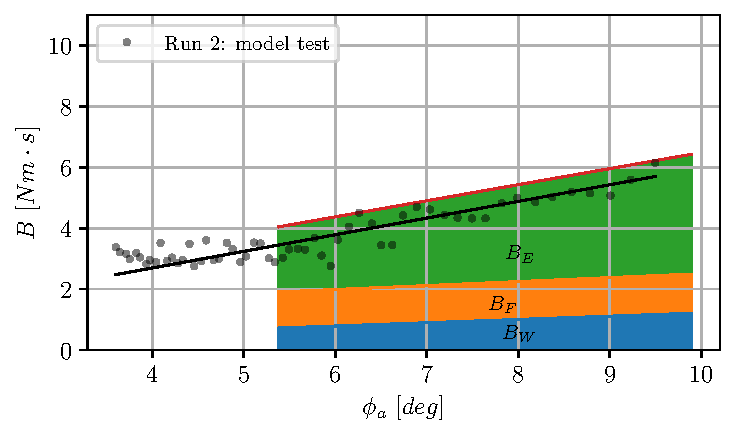
\includegraphics[width=\textwidth]{figures/hybrid_0.pdf}\end{center}
%\vspace{-0.4cm}
\caption{Roll damping from hybrid method ($F_n = 0$) for KVLCC2.}
\label{fig:hybrid_0}
\end{figure}
\begin{figure}[h]
\begin{center}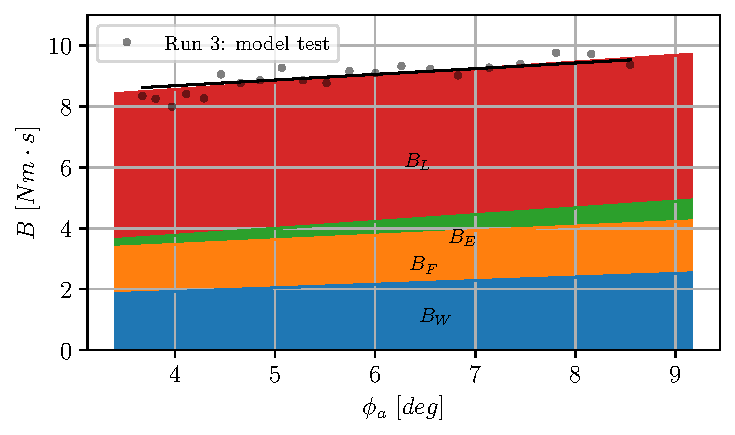
\includegraphics[width=\textwidth]{figures/hybrid_speed.pdf}\end{center}
%\vspace{-0.4cm}
\caption{Roll damping from hybrid method ($F_n = 0.14$) for KVLCC2.}
\label{fig:hybrid_speed}
\end{figure}
Roll decay simulations with damping from the hybrid method were conducted. Results from these simulations were compared with the model tests at zero speed (\autoref{fig:hybrid_0_time}) and at speed (\autoref{fig:hybrid_speed_time}). The time series from the corresponding FNPF
simulations have also been added to these plots to demonstrate the influence of the injection of semi-empirical viscous damping on the accuracy of these simulations.

Paper \ref{pap:ikeda} concluded that Ikeda's method offers an effective semi-empirical approach for predicting viscous roll damping. When combined with modern potential flow codes, such as FNPF, it enables highly accurate predictions of ship roll motion. 
\begin{figure}[h]
\center
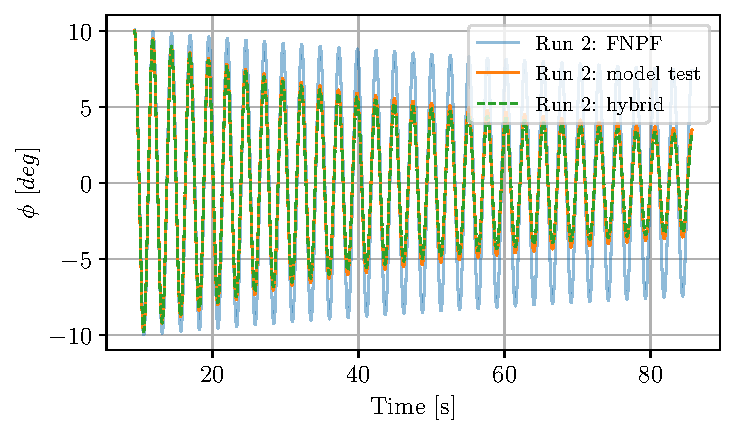
\includegraphics[width=\textwidth]{figures/hybrid_0_time.pdf}
%\vspace{-0.7cm}
\caption{Roll decay ($F_n=0$) for KVLCC2.}
\label{fig:hybrid_0_time}
\end{figure}
\begin{figure}[h]
\center
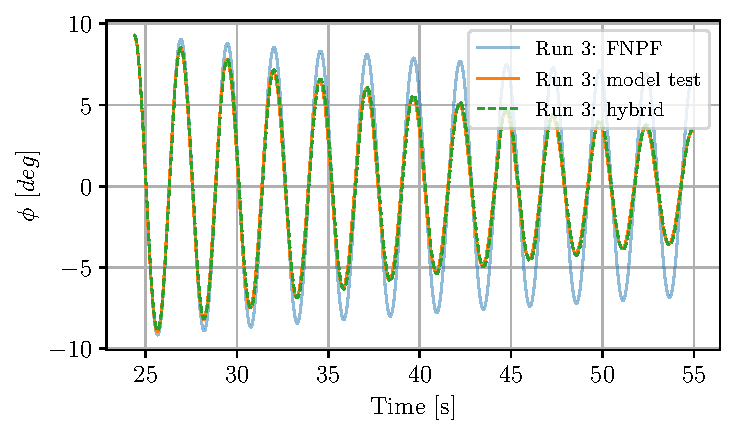
\includegraphics[width=\textwidth]{figures/hybrid_speed_time.pdf}
%\vspace{-0.7cm}
\caption{Roll decay ($F_n=0.14$) for KVLCC2.}
\label{fig:hybrid_speed_time}
\end{figure}